\section{Aufbau}
In Abbildung \ref{fig:Aufbau} ist das Interferometer mit dem Laser dargestellt. Der Detektionspfad zur Messung der Interferenzstrahlung ist nicht aufgezeigt.
\begin{figure}
  \centering
  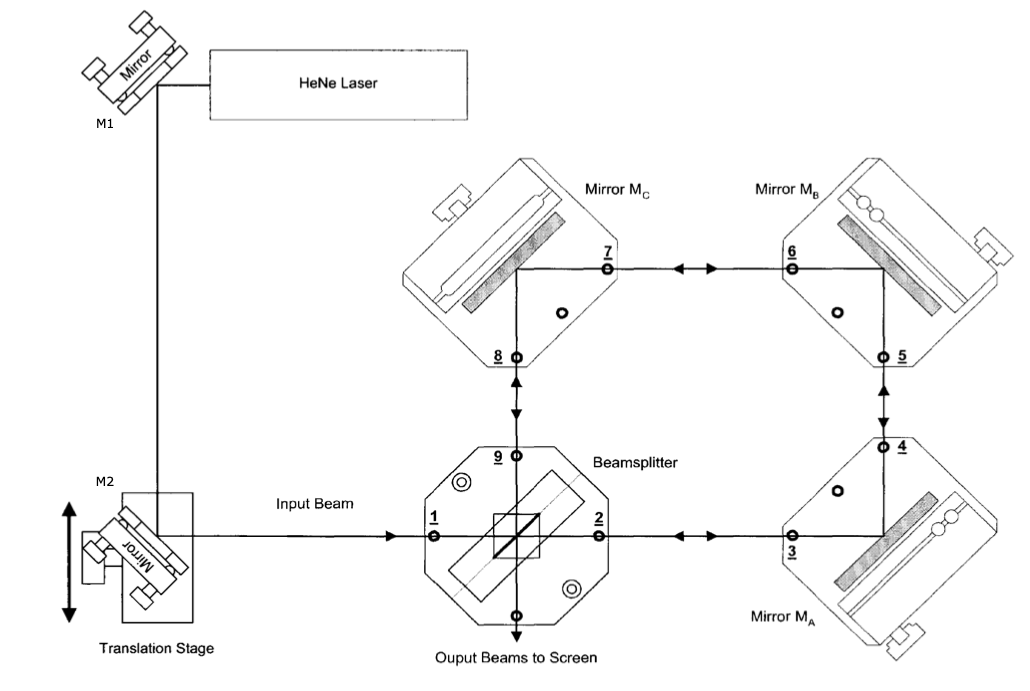
\includegraphics[width = .8\textwidth]{bilder/Aufbau.png}
  \caption{Aufbau des Sagnac-Interferometer ohne den Detektionspfad hinter dem PBSC (Punkt 10) \cite{anleitung}.}
  \label{fig:Aufbau}
\end{figure}
Als Strahlungsquelle des Sagnac-Interferometers dient ein \ce{HeNe}-Laser ($\lambda = \SI{632.99}{\nano\meter}$).
Der Laserstrahl wird zuerst durch zwei Spiegel auf einen Polarisationsfilter abgelenkt.
Mit dem Polarisationsfilter lässt sich aus dem linear polarisierten Laserstrahl eine Polarisationsrichtung auswählen.
Der Strahl trifft nach dem Polarisationsfilter auf den PBSC und wird dort nach seiner Polarisationsrichtung transmittiert (horizontale Polarisation), oder um \SI{90}{\degree} reflektiert (vertikale Polarisation).
Der weitere Aufbau ist geprägt durch 3 Spiegel, die mit dem PBSC ein Viereck bilden (vgl. Abbildung \ref{fig:Aufbau}).
Das vorher transmittierte Licht trifft somit an der Stelle auf den PBSC, an der das reflektierte Licht den PBSC verlassen hat und umgekehrt.
Somit werden sowohl transmittiertes und reflektiertes Lich nach ihrem Durchgang durch das Sagnac-Interferometer, wie zuvor, transmittiert und um \SI{90}{\degree} reflektiert.
\par\medskip
Weiterhin wird zur Erzeugung von Phasenverschiebungen eine Vorrichtung aus zwei Glasplättchen in den Strahlengang, zwischen Punkt 8 und 9, eingebaut.
Diese können, durch eine Drehscheibe, ihre Ausrichtung zum Strahlengang des Laserlichts verändern und so die Phasendifferenz beieinflussen.
Außerdem sind sie von ihrer Grundposition jeweils um einen festen Winkel gegen den Strahlengang gedreht.
\par\medskip
Für die Messung des Kontrastes des Interferometers unterscheidet sich der Aufbau von dem restlichen Versuchsteil.
Hinter dem PBSC wird im Detektionspfad ein weiterer Polarisationsfilter und hinter diesem eine Photodiode aufgebaut.
Dieser Polarisationsfilter sorgt dafür, dass nur die Polarisation einer bestimmten Richtung transmittiert wird und es so überhaupt zu Interferenzen kommt.
Um die benötigte Phasendifferenz für die Intensitäten $I_\text{min}$ und $I_\text{max.}$ zu erzeugen, wird der Strahlengang durch ein Verstellen des Spiegels M2 so auf den PBSC gelenkt, dass sich der Strahlengang örtlich aufteilt und auf die beiden Glasplättchen trifft.
Durch die Rotation dieser beiden Glasplättchen können die Intensitäten $I_\text{max.}$ und $I_\text{min.}$ für jeden Polarisationswinkel $\Theta$ des ersten Polarisationsfilters bestimmt werden und daraus der Kontrakt $K$ für diesen Polarisationswinkel bestimmt werden.
\par\medskip
Zur Messung des Brechungsindex der Glasplättchen wird im Detektionspfad statt dem Polarisationsfilters ein weiterer PBSC aufgebaut.
Sowohl das reflektierte Licht als auch das transmittierte Licht dieses PBSC trifft dann auf je eine Photodiode.
Aus der Differenzspannung der beiden Photodioden kann somit die Anzahl der $2\pi$ Phasenverschiebungen aus den Nulldulgängen bestimmt werden.
\par\smallskip
Der selbe Aufbau des Detektionspfads wird auch für die Messung der Brechungsindex für Luft in Abhängigkeit des Luftdrucks genutzt.
Die Glasplättchen werden aus den beiden Strahlen entfernt und dafür eine Druckkammer in einen der beiden Strahlen gestellt.
Der Druck in der Druckkammer kann durch eine Vakuumpumpe reduziert und über ein Ventil mit Luft geflutet werden.
